\chapter{Implementation}
\index{implementation}

\section{Allocation}
\label{allocation}

As for any filesystem, \wi{fragmentation} hurts performance and therefore is preferably kept at a minimal level. This is especially true for our filesystem, since we have a maximum number of extents which can be stored within an inode, as outlined in section \ref{fileinode}.

In order to work around this, we use a different allocation strategy:

\begin{itemize}
\item Random first blocks \\
For every first file block, we take a random block somewhere within the free space list of our disk.
\item Extend previous blocks \\
If we have a previously allocated block, we try to take the next block. If this fails, we take a random block.
\end{itemize}

Support we have the layout as below, \emph{a} and \emph{b} are files. The text below the image is the extent map as stored within the FIT:

\begin{figure}[h]
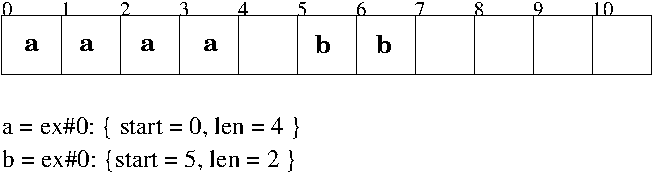
\includegraphics[width=10cm]{alloc1}
\caption{Allocation strategy: initial status}
\end{figure}

Now, let's assume we allocate an extra block for file \emph{a}. Since there is a free block coming ahead, we can easily expand the extend. This gives the following:

\begin{figure}[h]
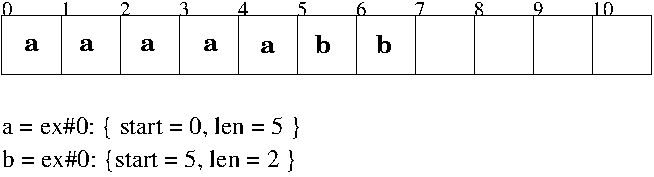
\includegraphics[width=10cm]{alloc2}
\caption{Allocation strategy: after extending file 'a'}
\end{figure}

However, suppose file \emph{a} wants another block. It may not overwrite the blocks already in use by file \emph{b}, so we allocate a random block:

\begin{figure}[h]
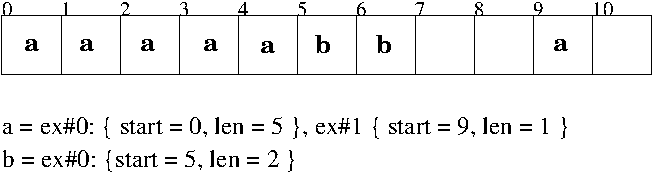
\includegraphics[width=10cm]{alloc3}
\caption{Allocation strategy: after extending file 'a' again}
\end{figure}

Finally, let's assume we create a new file, \emph{c}, with a single block. This block will be randomly put somewhere on the disk:

\begin{figure}[h]
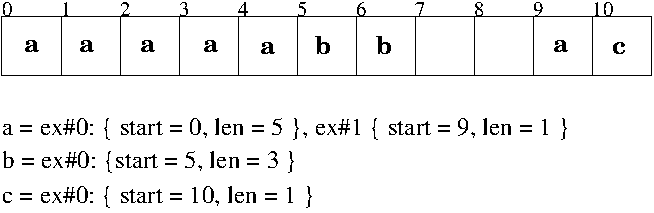
\includegraphics[width=10cm]{alloc4}
\caption{Allocation strategy: new file 'c' with a data block}
\end{figure}

As can be seen, this hinders file \emph{a} since it cannot extend to the next block and thus must create a new extent.

\section{Free space}
\label{freespace}

\subsection{Introduction}

Unlike most traditional filesystems, LIMEFS does not store an overview of free blocks on the disk. Rather, this list is constructed upon mount time and consists of the following characteristics:

\begin{itemize}
\item Stored as an extent list \\
In order to allow quick access, the freelist is stored as an extent-based list.
\item Numerically sorted \\
The list is always numerically sorted. This simplifies merging adjacent blocks.
\item Limited number of entries \\
The maximum list size\footnote{This will happen if even numbered blocks are used whereas odd numbered blocks are free} is $\frac{numDataBlocks}{2}$. Tests have shown this never happens, so we use a tenth of the maximum, or $\frac{numDataBlocks}{10}$.
\end{itemize}

These characteristics will be illustrated in the next paragraph.

\subsection{Example}

Below is an example of a free list. Shaded blocks lines are allocated, blank blocks are available:

\begin{figure}[h]
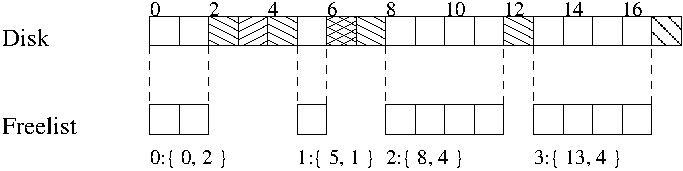
\includegraphics[width=12cm]{freelist1}
\caption{Freelist: initial status}
\end{figure}

Now, we free block 3. This means we need to add an extra entry to our freelist (since it is in the middle of used blocks. This gives the following:

\begin{figure}[h]
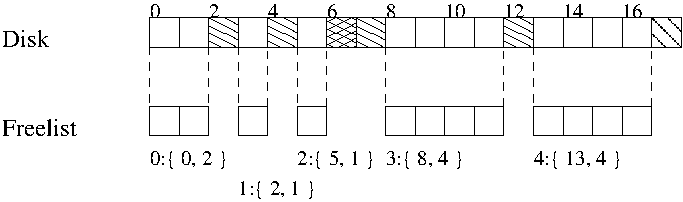
\includegraphics[width=12cm]{freelist2}
\caption{Freelist: freed block 3, gives new extent}
\end{figure}

\newpage

Block ranges can also be extended. For example, if we free block 6, we get:

\begin{figure}[h]
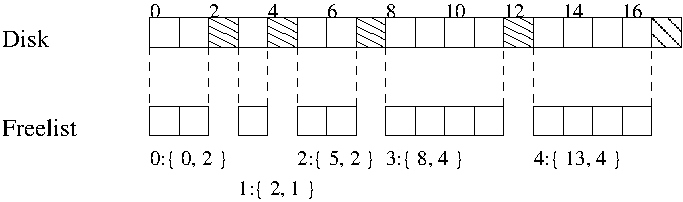
\includegraphics[width=12cm]{freelist3}
\caption{Freelist: freed block 6, expands extent}
\end{figure}

Finally, entire freelist extents can get merged. Suppose we free block 12, we get:

\begin{figure}[h]
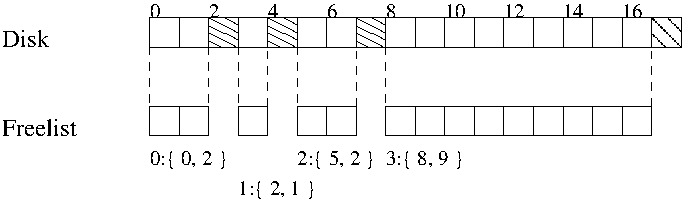
\includegraphics[width=12cm]{freelist4}
\caption{Freelist: freed block 12, merges extents}
\end{figure}

\subsection{Operations}

Only two operations need to be implemented by the freelist:

\begin{itemize}
\item Add a block to the freelist \\
This is done by \texttt{lime\_extent\_mergefreeblocks}, which adds a previously-allocated block to the free list.
\item Remove free block from the list \\
Done by \texttt{lime\_extent\_removefreeblocks}, this will remove the blocknumber from the list.
\end{itemize}

These functions can be found in \texttt{fs/lime/freelist.c}.

\section{Locking}

From Linux 2.0 onward, there has been support for multiple processors. This used to be implemented using a single lock, but as it matured, finer-grained locking is used to protect data structures.

\standon{Kernel-side locks in Linux}{Kernel-side locks}

As outlined in \cite{LKD}, chapter 9, we could use the following locks:

\begin{itemize}
\item \wi{Atomic bitwise operations} \\
Linux 2.6 provides atomic bitwise set, clear and retrieve bit operations. These are useful for maintaining flags.
\item \wi{Spinlocks} \\
A spin lock is an inexpensive operation, which will keep a CPU waiting (spinning) to see if a lock can be obtained. It will wait until it can. This is useful for data structures, but it may never be used if a context switch could occur.
\item \wi{Reader/writer spinlocks} \\
This is the same as an ordinary spinlock, except that you lock for reading or writing. Multiple readers will be allowed, but there may be only one writer and never a writer if there are readers.
\item \wi{Semaphores} \\
Semaphores are locks which can be held while blocking. This is useful for long sleeps (such as while passing data from or to userland).
\end{itemize}
\standoff

Since you can not hold semaphores in an interrupt context and no spinlocks while doing a context switch, it is important to determine which lock to use. The codebase uses read/write spinlocks for the FIT and freelist\footnote{Writes are much more rare than reads, and it would be a waste of resources to wait to let readers spin if no one is writing}, and atomic bitwise operations for the flags variable. The superblock does not have a lock because it is readonly, as outlined in section \ref{superblock}.

\section{Hard links}
\label{impl_hardlinks}

As outlined in section \ref{hardlink}, hardlinks are supported. However, they need special treatment on this filesystem, due to the fact that no reference counts are maintained. Since the FIT is maintained entirely within memory, this operation is relatively inexpensive.

Whenever a hardlink is created, it is like a normal inode, which contains the destination inode number. Inode reads will notice this is a hardlink, and refer to the hardlinked file.

Deletion is different. A hardlink itself can always be deleted without any problems. However, whenever a file is deleted, it must be known whether any hard links refer to the file. If this is the case, the hardlink's filename is simply copied over the original file and the hardlink inode is removed instead of the original file to be deleted.

\section{Begin and end offsets}
\label{impl_offs}

As outlined in section \ref{offs}, the filesystem supports begin and end offsets in order to allow truncation of a file. This truncation can occur from the begging of the file or from the end of the file, refer to section \ref{offs} for more information. Within the filesystem, the \texttt{boff} offset is simply added to the offset the user wants to read.

This has a severe limitation, namely that \texttt{boff} must be in disk blocks as only disk block-sized blocks can be read. The only way around this would be, to read 2 diskblocks and merge them. Since this cannot be done using traditional buffer cache functionality, which assumes one block is one buffer, a lot of existing code would have to be duplicated.

\section{Commit daemon}

A filesystem must always ensure reasonable integrity. Since all meta data is kept in-memory for this filesystem, a powerloss would mean the filesystem's FIT would be identical to the one on disk when we first mounted the filesystem. However, this would not be in sync with the file contents on disk.

In order to work around this, we periodically flush (commit) the FIT structure to the disk. Since we have 2 copies of the FIT (refer to section \ref{fit} for more information), a crash while writing the FIT means no data loss (except for data written after the last commit, of course).

This \wi{commit daemon} is implemented as a kernel thread, since we need to hold separate locks. A bit in the flags register is used to mark the FIT as dirty, this bit is cleared after the new FIT is committed to disk. Upon unmounting of the filesystem, a special unmount flag is set and the commit daemon is signaled to wake up. It will do a final flush if the FIT is dirty, and exit.

The implementation of the daemon can be found in \texttt{fs/lime/fit.c}, in the function \texttt{lime\_commitd}.

\section{Tests}

This is an Extreme Programming project, which means software tests are created beforehand in order to maintain a consistent level of quality. Since this is a kernel module, subsystems are hard to test using conventional tests.

To overcome this, the freelist implementation can be compiled in userland and kernelspace. Using standard testing libraries, the freelist is filled and the structures are compared to what they should be. This provides easy validation, since freelist corruption is much harder to debug when it occurs in kernelspace.

Finally, tests have been created to ensure proper operation of the filesystem by creating, deleting, writing and reading files, creating/removing directories, using links and such. Even though not all cases can possibly be tested, most tests try to provide the necessary complexity to increase the chance to trigger a failure.

All tests can be found in the \texttt{lime-linux/test} directory.
